\chapter{Topology}

Topology is a minimal amount of structure put onto sets.  Once we have sets, we can start arranging the objects in them and assigning more information to the objects in the sets.

\begin{definition}[Topological Space] \label{def:topspace}
  A \textbf{Topological Space} is a set $X$ and a collection of subsets of $X$, $T$, such that
  \begin{enumerate}
    \item The empty set $\varnothing \in T$.
    \item $X \in T$.
    \item The intersection of a \textit{finite} number of sets in $T$ is also in $T$.
      \begin{equation}
        \cap_{T_i\in T}^{N < \infty} T_i \in T
      \end{equation}
    \item The union of \textit{up to an infinite number} of sets in $T$ is also in $T$.
      \begin{equation}
        \cup_{T_i \in T} T_i \in T
      \end{equation}
  \end{enumerate}
\end{definition}

\begin{example}[Trivial Topology]\label{ex:trivialtop} A \textbf{Trivial Topology} is when, for a given set $X$, the topology only contains $X$ and the null set $\varnothing$.

\begin{center}
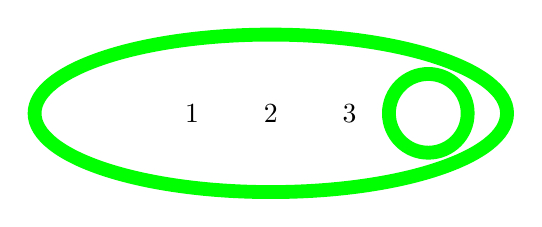
\begin{tikzpicture}
    \draw (-1,0) node{1};
    \draw (0,0) node{2};
    \draw (1,0) node{3};
    \draw[green, line width=5] (0,0) circle [ x radius = 3, y radius = 1];
    \draw[green, line width=5] (2,0) circle [x radius =.5, y radius = .5];
\end{tikzpicture}\end{center}
\end{example}

\begin{example}[Discrete Topology]\label{ex:discretetop} For a given set $X$, its \textbf{discrete topology} is the collection of all subsets of $X$.

\begin{center}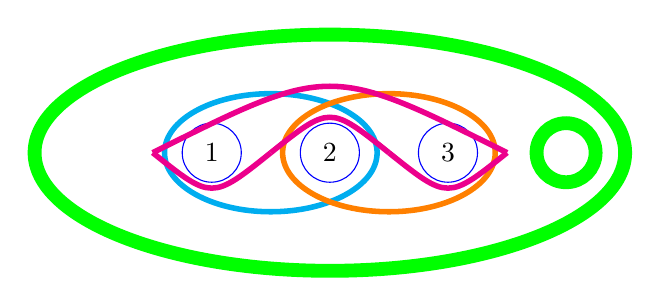
\begin{tikzpicture}[scale=1.5]
    \draw (-1,0) node{1};
    \draw (0,0) node{2};
    \draw (1,0) node{3};
    \draw[green, line width=5] (0,0) circle [ x radius = 2.5, y radius = 1];

    \draw[blue] (-1,0) circle [x radius =.25, y radius = .25];
    \draw[blue] (0,0) circle [x radius =.25, y radius = .25];
    \draw[blue] (1,0) circle [x radius =.25, y radius = .25];

    \draw[cyan, line width=2pt] (-.5,0) circle [x radius =.9, y radius = .5];
    \draw[orange, line width=2pt] (0.5,0) circle [x radius =.9, y radius = .5];

    \draw[magenta, line width=2pt] (-1.5,0) .. controls (0,.75) .. (1.5,0);
    \draw[magenta, line width=2pt] (-1.5,0) .. controls (-1, -.4) .. (-.5,0);
    \draw[magenta, line width=2pt] (-.5,0) .. controls (0,.4) .. (.5,0);
    \draw[magenta, line width=2pt] (.5,0) .. controls (1,-.4) .. (1.5,0);

    \draw[green, line width=5] (2,0) circle [x radius =.25, y radius = .25];
\end{tikzpicture}\end{center}
\end{example}

\begin{example}\label{ex:neithertop} Here's an example of a 3-element set that is neither the trivial nor discrete topology.

\begin{center}  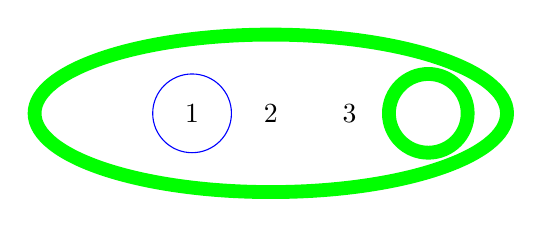
\begin{tikzpicture}
      \draw (-1,0) node{1};
      \draw (0,0) node{2};
      \draw (1,0) node{3};
      \draw[green, line width=5] (0,0) circle [ x radius = 3, y radius = 1];
      \draw[green, line width=5] (2,0) circle [x radius =.5, y radius = .5];

      \draw[blue] (-1,0) circle [x radius =.5, y radius = .5];
  \end{tikzpicture}\end{center}
\end{example}

We can also have topological spaces for continuous sets, like $\mathbb{R}$ or $\mathcal{S}^1$.

\begin{definition}[Open Ball]
  For $\epsilon > 0$, an \textbf{open ball} at point $p_1$ of radius $\epsilon$ is all points $B_{\epsilon}(p_1)= \{p_i | \abs{p_i - p_1}<\epsilon \}$.
\end{definition}

\begin{definition}[Standard Topology] \label{def:standardtop}
  The \textbf{Standard Topology} for a given set $X$ is the set, the null set, all open balls, and all finite unions of open balls.
\end{definition}

The standard topology is quite useful for limits and Calculus, since for any $\epsilon >0$, we can always find points $p_1, p_2$ such that $\abs{p_1 - p_2} <\epsilon$.

\section{Comparing Topologies}
In Section~\ref{sec:comp}, we defined two terms for comparing sets with an algebraic structure, \textit{homomorphism} and \textit{isomorphism}.  After we have attached a topology to the set, we have two analogous concepts with very confusing terminology.788

\begin{definition}[Homotopic]
  Two topologies are \textbf{homotopic} to each other if one can be continuously deformed into another, allowing for the collapse of dimensions and information loss.

  Officially, if there exists a function $F:X\times[0,1] \rightarrow Y$ that is continuous, then $X$ and $Y$ are homotopic.
\end{definition}

\begin{definition}[Homeomorphism]
  Two topologies $X$ and $Y$ are \textbf{homeomorphic} if there exists a function $f: X \rightarrow Y$ and inverse function $f^{-1}: Y \rightarrow X$ that are both continuous.
\end{definition}

The difference between \textit{homomorphic, homoemoprhic,} and \textit{homotopic} is tricky.  \textit{Homomorphic} and \textit{Isomorphic} are general categorization terms that apply to sets, research \textbf{Category Theory} for more information.  \textit{Hom\textbf{E}omorphic} applies specifically to topolog\textbf{Y} and geometr\textbf{Y}.

\section{Properties of Topologies}

While to prove two topologies homeomorphic, we need to find a map $f$ between them and it's inverse, we have more painless ways to prove that two topologies are not homeomorphic.  We have properties of topologies that are held invariant under isomorphism.  If we can show that two different topologies have different properties, then we know that they can't be isomorphic to each other.  If two topologies agree on every known property, then they probably are isomorphic to each other, but mathematicians love their counterexamples, so don't count on it.



\begin{definition}[Compact]
  A topology is called \textbf{compact} if every open cover has a finite subcover.
\end{definition}
That was the formal definition, but what does it mean?  Sometimes my desk seems like it has an infinite amount of papers spread out over it.  Let us suppose that my desk literally does have an infinite number of papers covering it.  I could take either a finite number of papers or an infinite number of papers to cover my desk, but either way, I could always find a finite subset of those that still cover the desk.

As opposed to my desk, the real line with the standard topology is not compact.  Suppose I choose the infinite cover of the real line $\mathbb{R}$,

\begin{center}
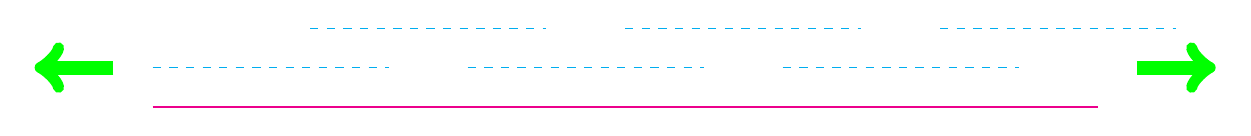
\begin{tikzpicture}[scale=2]
  \draw[green,->, line width=5] (-.25,.25) --  (-.75,.25);
  \draw[green,->, line width=5] (6.25,.25) -- (6.75,.25);
  \draw[magenta] (0,0) -- (6,0);
  \foreach \x in {0, 2, 4}
  { \draw[cyan, dashed] (\x,.25) -- (\x + 1.5,.25);
    \draw[cyan, dashed] (\x +1,.5) -- (\x +2.5,.5);}
\end{tikzpicture}
\end{center}

I have covered the real line with an infinite number of sets, but if I take even one away, $\mathbb{R}$ will no longer be covered.  The cover presented above does not have a \textit{finite} subcover.  Since \textit{every} cover has to have a finite subcover for a topology to be compact, we just to show one counter-example to show that a topology is not compact.  Hence, Reals equipped with the standard topology is not compact. QED.

Quod Erat Demonstrandum. Not Quantum Electro-Dynamics.  Much as I like me some relativistic light-matter interactions.

Moral of the story: don't play strip poker with the Real Numbers. If they started covered up, no matter how much they lose, there would always be more clothing to remove.

\begin{definition}[Hausdorff]
    Also known as \textbf{$T_2$}, every two points in a \textbf{Hausdorff} space have disjoint neighborhoods.
\end{definition}

\begin{definition}[Orientable]
  A topological space of dimension $n$ is said to be \textbf{Orientable} is it can be covered by a nowhere vanishing $n$-form.
\end{definition}
This $n$-form could potentially be the orientation of the space, though others might exist.



\subsection{Euler Character and Gauss-Bonnett Formula}

\section{Coordinate Systems}
Once we have a topology for a set, we can put even more information on the object via a coordinate system. At least in some circumstances. A topology gave us an idea of which objects are ``neighbors" and ``next to each other".  If two objects are usually in subsets together, then they are adjacent.  A coordinate system gives a precise way to quantify this.

So in what circumstances can we do this? When we are dealing with a \textbf{manifold}.

\begin{definition}[locally]
   If a condition holds \textbf{locally}, then for every point $p\in X$, $p$ is in some open set such that the condition holds on that open set.
\end{definition}

\begin{definition}[Manifold]
A \textbf{Manifold} is a topological space that locally looks like Euclidean space, $\mathbb{R}^n$, for some $n$.
\end{definition}

 The Standard Topology, ex.~\ref{def:standardtop}, could be a manifold, depending on the underlying set. For example, $X=\mathbb{R}$ equipped with the standard topology is a manifold, but the standard topology on a set like

\begin{center}
  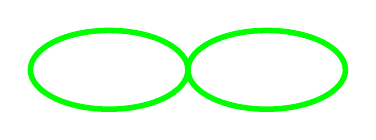
\begin{tikzpicture}
    \draw[line width=2, green] (-1,0) circle [x radius =1, y radius = .5];
    \draw[line width=2, green] (1, 0) circle [x radius =1, y radius = .5];
  \end{tikzpicture}
\end{center}

  is not a manifold because the point where the circles are joined no longer looks like a line.  Our other previous examples, ex.~\ref{ex:trivialtop},~\ref{ex:discretetop}, and \ref{ex:neithertop} are not manifolds as they are discrete.

\begin{definition}[Coordinate Chart]
  A \textbf{Chart} of a topology is a map $\phi: U \rightarrow V$, where $U$ is an open set in the topology, and $V$ is an open set in $\mathbb{R}^n$.   $\phi$ must be one-to-one and onto, thus defining a homeomorphism.
\end{definition}

\begin{definition}[Atlas]
  An \textbf{Atlas} is a collection of charts covering the entirety of a topological space.  If two charts overlap on a set $U \cap V$, where $\phi:U\rightarrow \mathbb{R}^n$ and $\psi:V\rightarrow \mathbb{R}^n$, then the transition function $\phi \circ \psi^{-1}: \mathbb{R}^n \rightarrow \mathbb{R}^n$ must be defined on $U\cap V$, be continuous, and be differentiable.
\end{definition}

See Fig~\ref{fig:atlas} for a conceptual idea of what an atlas and charts are.  While the mathematical terminology might seem strange and at odds with our conception from the English terms, the mathematical abstraction and everyday object have much in common.  The atlas is the comprehensive book of everything put together, all the charts.  We need more than one chart because I don't want United States highways at the same time I'm planning how to get around on the Tokyo subway.  Also, because latitude and longitude are ill-defined on the north pole.


\begin{figure}
  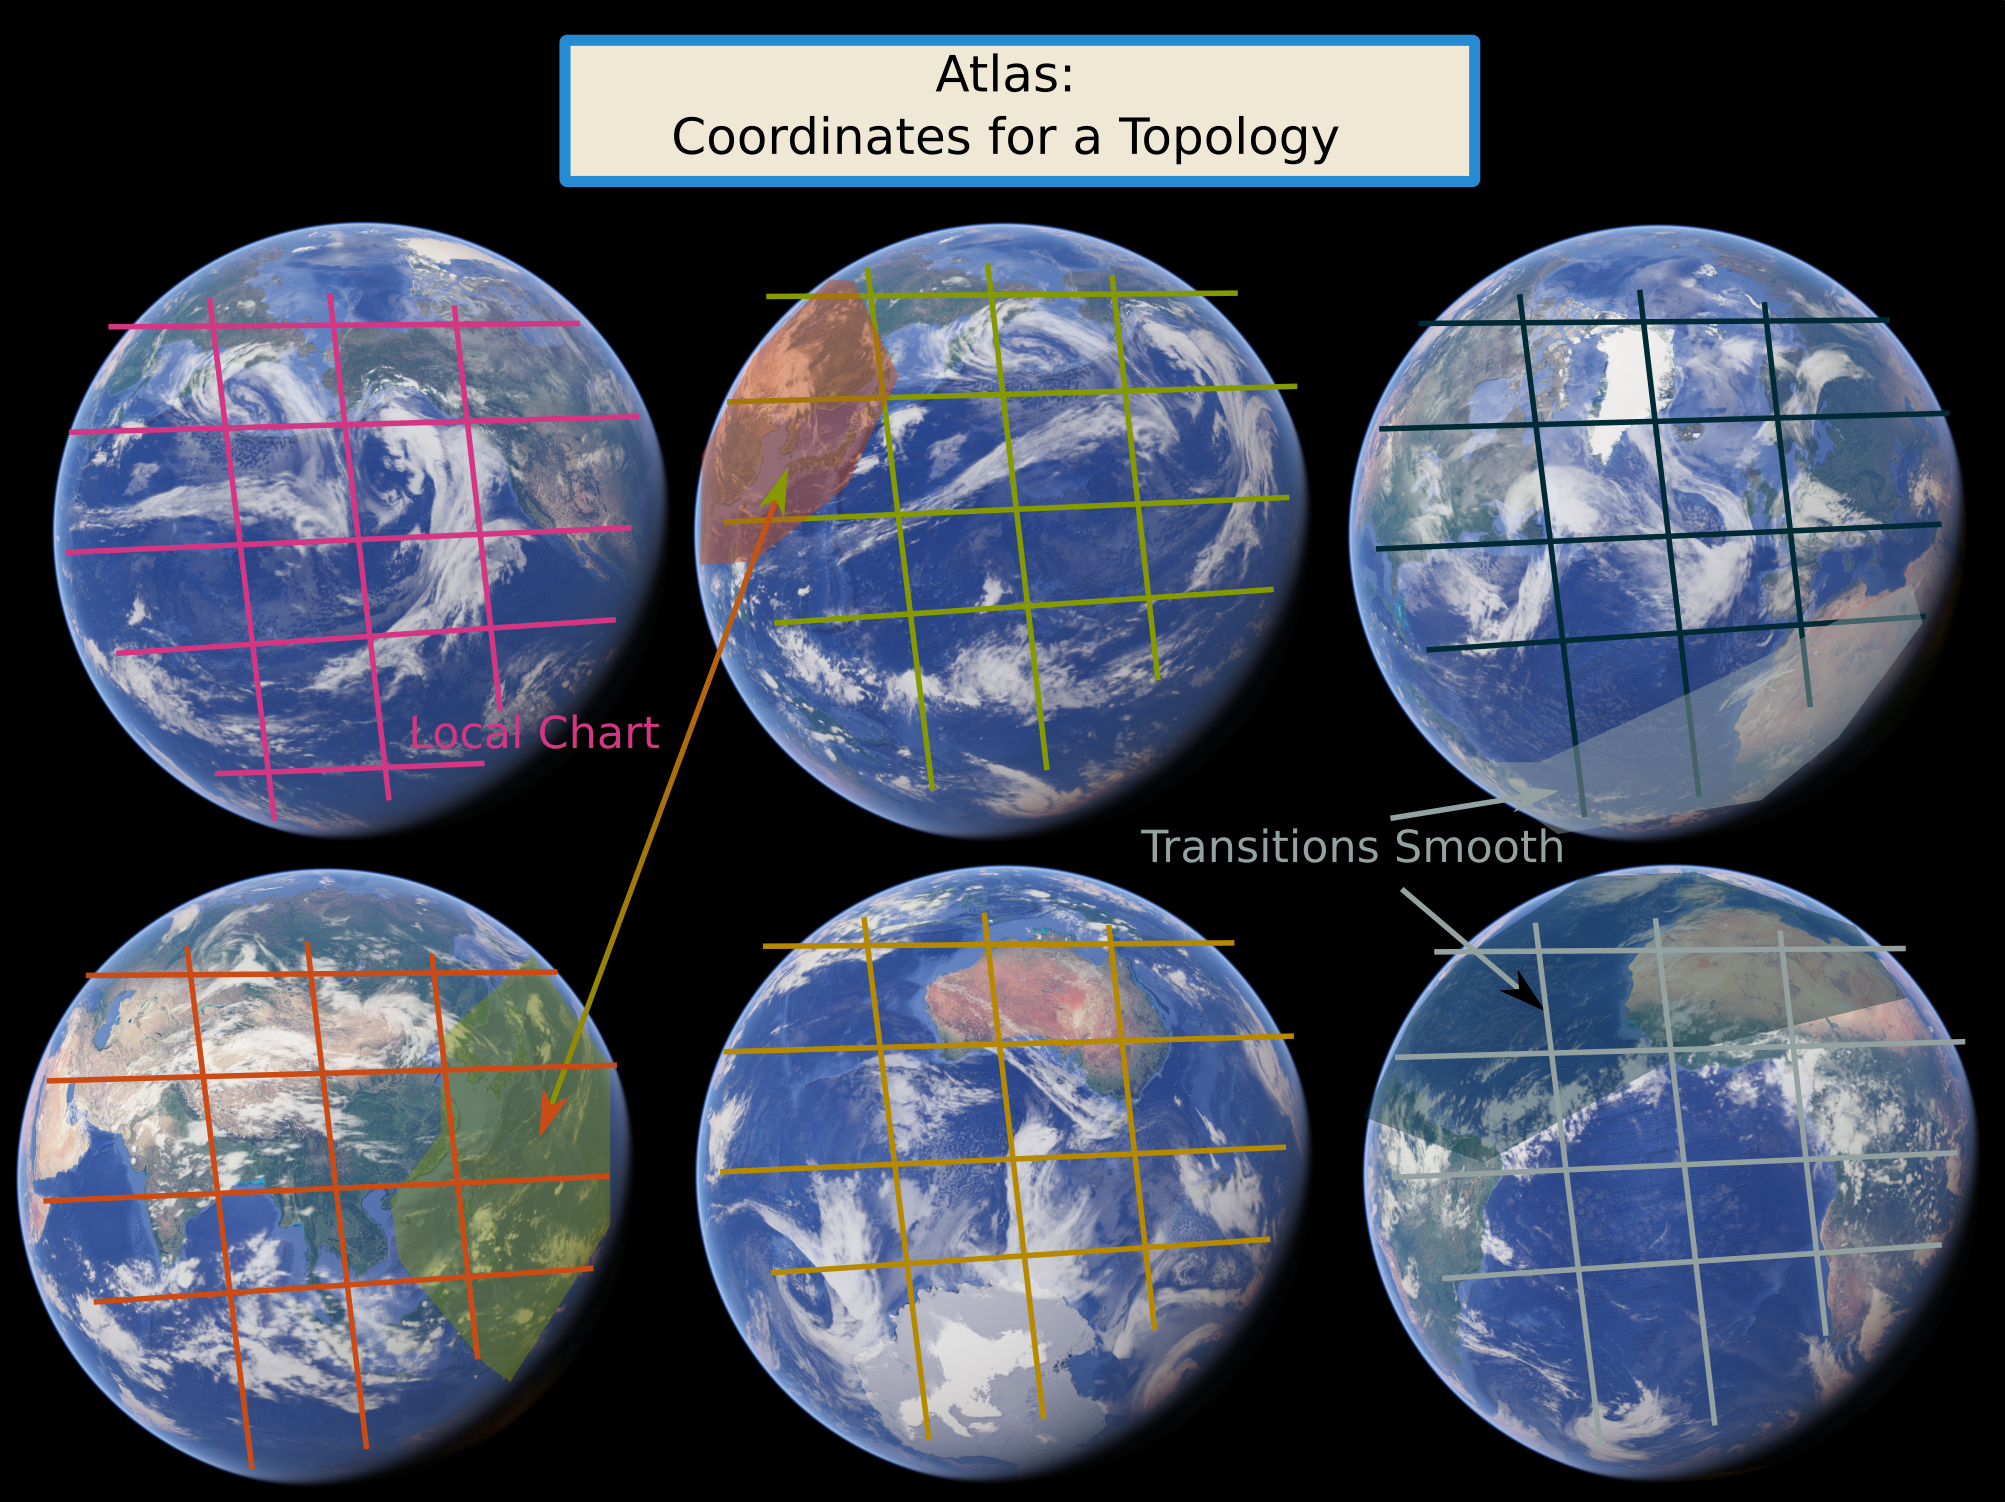
\includegraphics[width=\textwidth]{pics/atlas.png}
  \caption{An atlas is composed of sets which possess coordinate systems, and smooth transition functions between the coordinate systems where the sets overlap.}
    \label{fig:atlas}
\end{figure}
